\begin{figure}\centering\scriptsize
    \begin{subfigure}{0.48\textwidth}\centering
        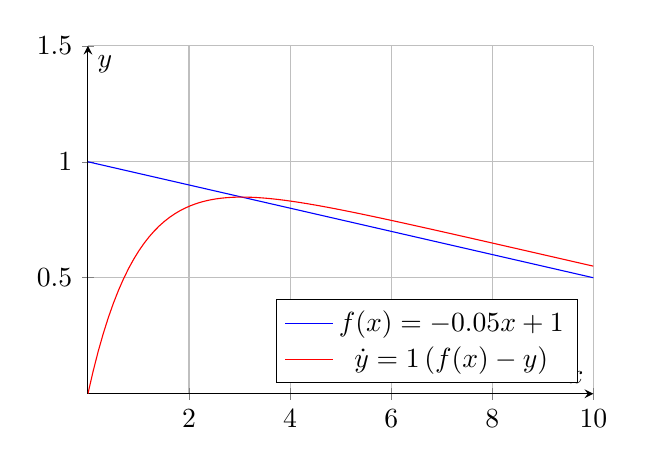
\begin{tikzpicture}
            \begin{axis}[axis lines=middle,xlabel=$x$,ylabel=$y$,grid=both,width=8cm,height=6cm,legend pos=south east,ymin=0,ymax=1.5]
                \pgfmathsetmacro{\aa}{-.05}
                \pgfmathsetmacro{\bb}{1}
                \pgfmathsetmacro{\cc}{1}
                \addplot[domain=0:10,samples=100,color=blue]{\aa*x+\bb};
                \addplot[domain=0:10,samples=100,color=red]{\aa*x+\bb+(\aa/\cc-\bb)*exp(-\cc*x)-\aa/\cc};
                \addlegendentry{$f(x)=\aa{}x+\bb$}
                \addlegendentry{$\dot{y}=\cc\left(f(x)-y\right)$}
            \end{axis}
        \end{tikzpicture}
    \end{subfigure}\hfill
    \begin{subfigure}{0.48\textwidth}\centering
        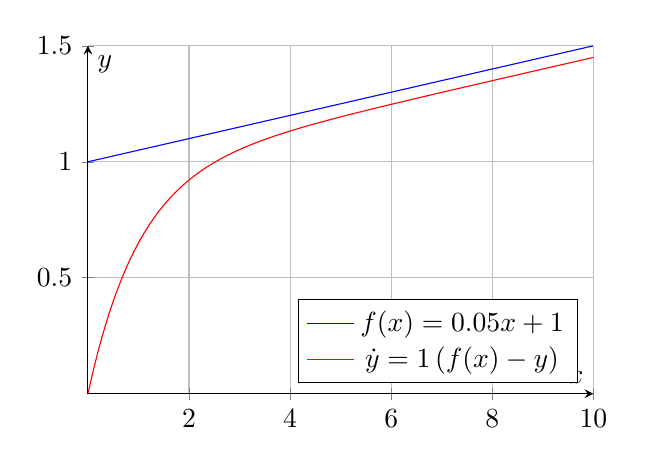
\begin{tikzpicture}
            \begin{axis}[axis lines=middle,xlabel=$x$,ylabel=$y$,grid=both,width=8cm,height=6cm,legend pos=south east,ymin=0,ymax=1.5]
                \pgfmathsetmacro{\aa}{0.05}
                \pgfmathsetmacro{\bb}{1}
                \pgfmathsetmacro{\cc}{1}
                \addplot[domain=0:10,samples=100,color=blue]{\aa*x+\bb};
                \addplot[domain=0:10,samples=100,color=red]{\aa*x+\bb+(\aa/\cc-\bb)*exp(-\cc*x)-\aa/\cc};
                \addlegendentry{$f(x)=\aa{}x+\bb$}
                \addlegendentry{$\dot{y}=\cc\left(f(x)-y\right)$}
            \end{axis}
        \end{tikzpicture}
    \end{subfigure}
\end{figure}